\section{Supplementary Comparisons}\label{app:supplement}
\subsection{Communication-round results versus local computation}
\Cref{fig:cost} compares the six settings by cumulative client-epochs. Unequal client sizes make sample exposures in \cref{tab:grid} a more precise computation measure.

One float32 model occupies $108{,}478\times4=433{,}912$ parameter bytes. An uncompressed download-plus-upload proxy is $2mT(433{,}912)$ bytes for $m$ participants and $T$ rounds, excluding protocol overhead and retries.
\begin{figure}[htbp]
\centering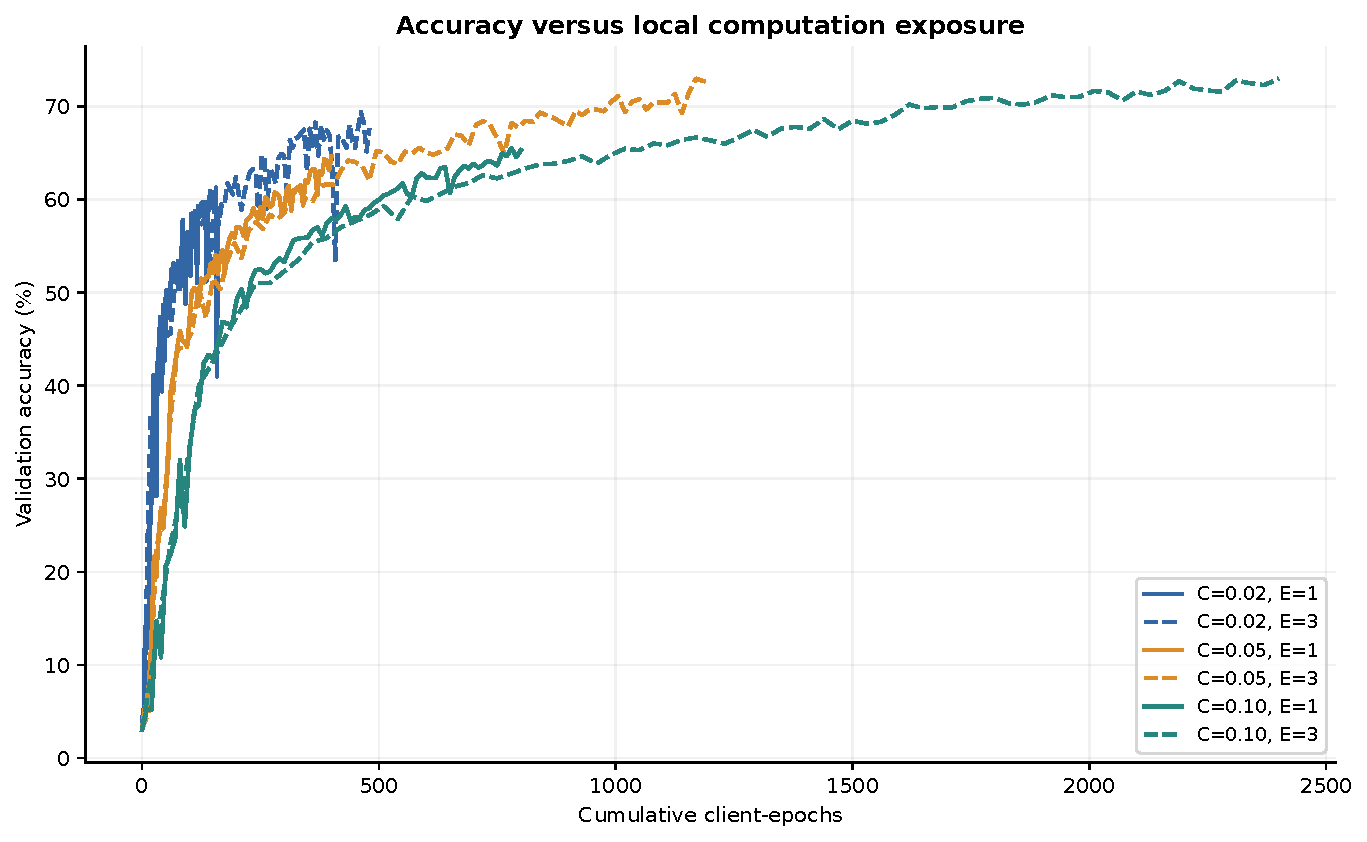
\includegraphics[width=0.9\linewidth]{figures/part1_1/accuracy_vs_client_epochs.pdf}
\caption{Validation accuracy versus cumulative client-epochs for the six seed-2026 configurations. Curves terminate at different budgets because all runs stop after 80 rounds.}\label{fig:cost}
\end{figure}

\subsection{Seed variability in the leading FedAvg settings}
\Cref{fig:seeds} shows pointwise mean validation accuracy and sample SD across three fixed-split seeds. Selection uses mean best validation across seeds, rather than the best point of this mean trajectory.
\begin{figure}[htbp]
\centering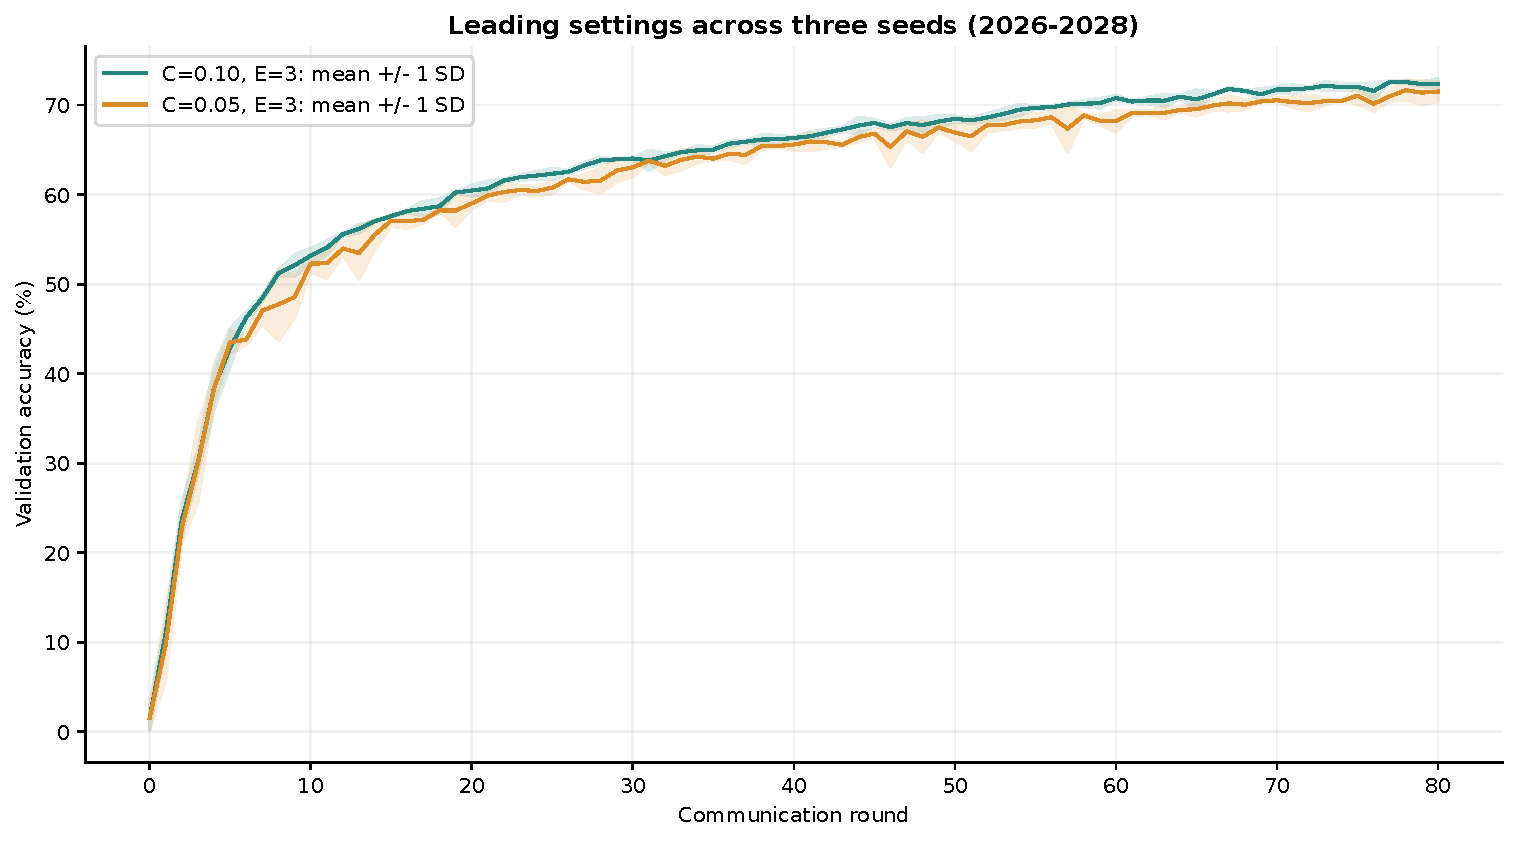
\includegraphics[width=0.9\linewidth]{figures/part1_1/seed_stability.pdf}
\caption{Leading sequential settings at $E=3$, seeds 2026--2028. Shading is one pointwise sample SD; the split remains fixed.}\label{fig:seeds}
\end{figure}

\subsection{Matched serial and Ray trajectories}
\Cref{fig:raymatch} displays the matched four-client CPU comparison: training and validation trajectories coincide, with maximum metric difference 0.0.
\begin{figure}[htbp]
\centering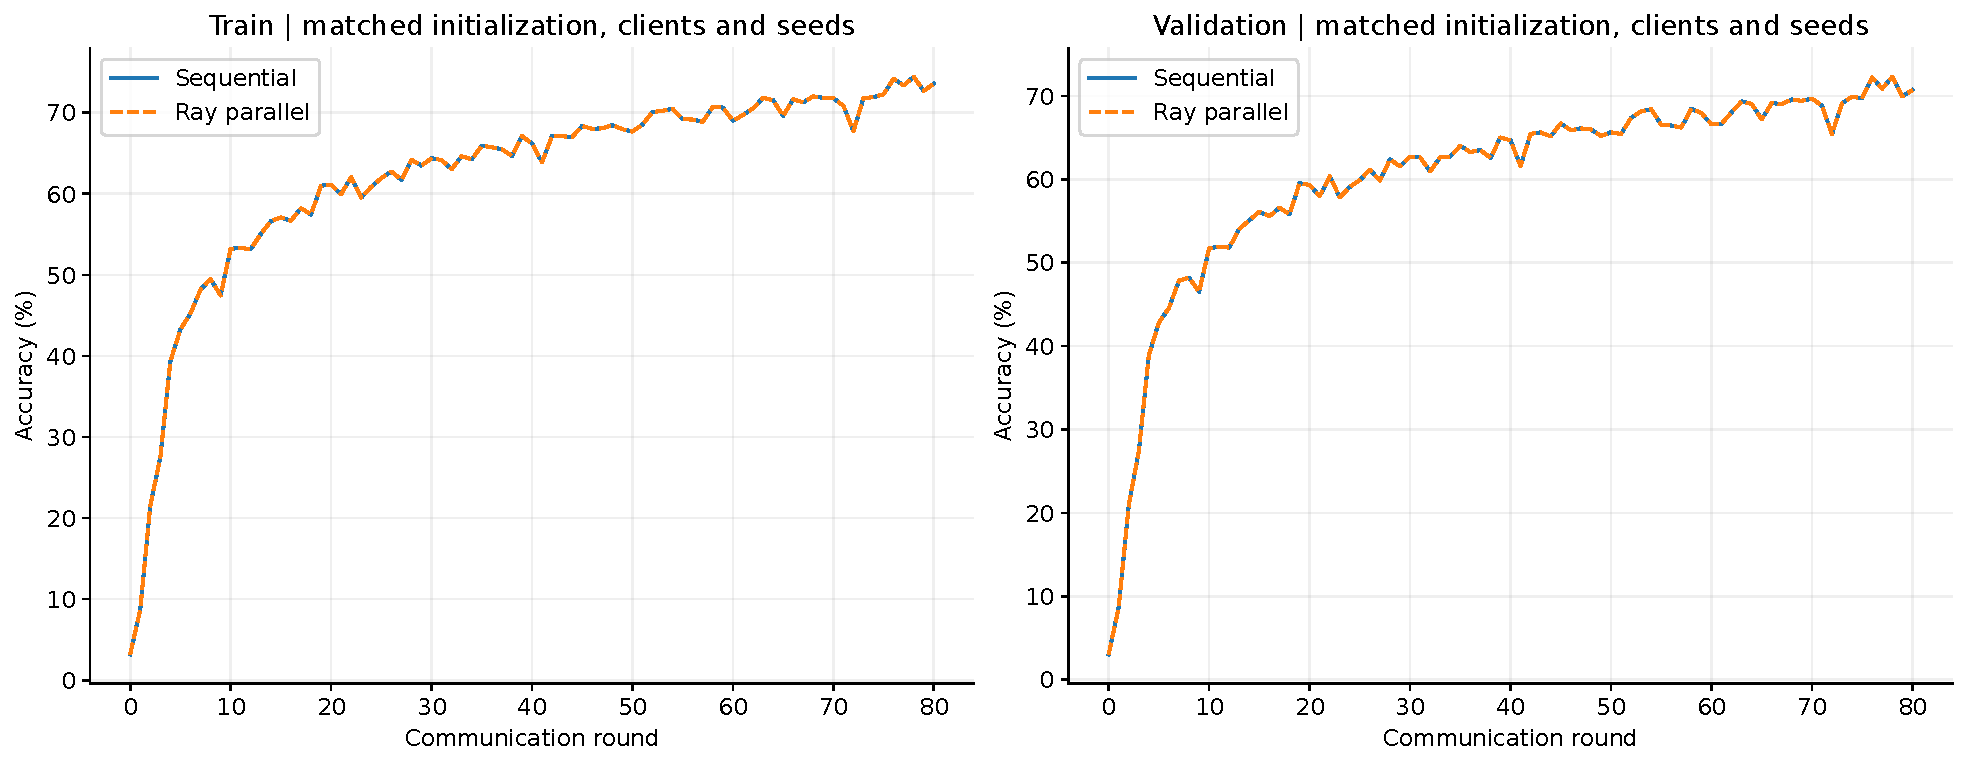
\includegraphics[width=\linewidth]{figures/part1_2/sequential_parallel_accuracy.pdf}
\caption{Matched 80-round sequential and Ray CPU accuracy trajectories, seed 2026, four clients per round. Initial parameters, selections, local minibatches, optimizer settings, and aggregation order are identical.}\label{fig:raymatch}
\end{figure}

\subsection{Distortion is a mechanism diagnostic, not a privacy budget}
\Cref{fig:distortion} relates measured RMS to $\sqrt{2}b$ and mean validation accuracy. Its horizontal axis is perturbation magnitude, not a privacy budget.
\begin{figure}[htbp]
\centering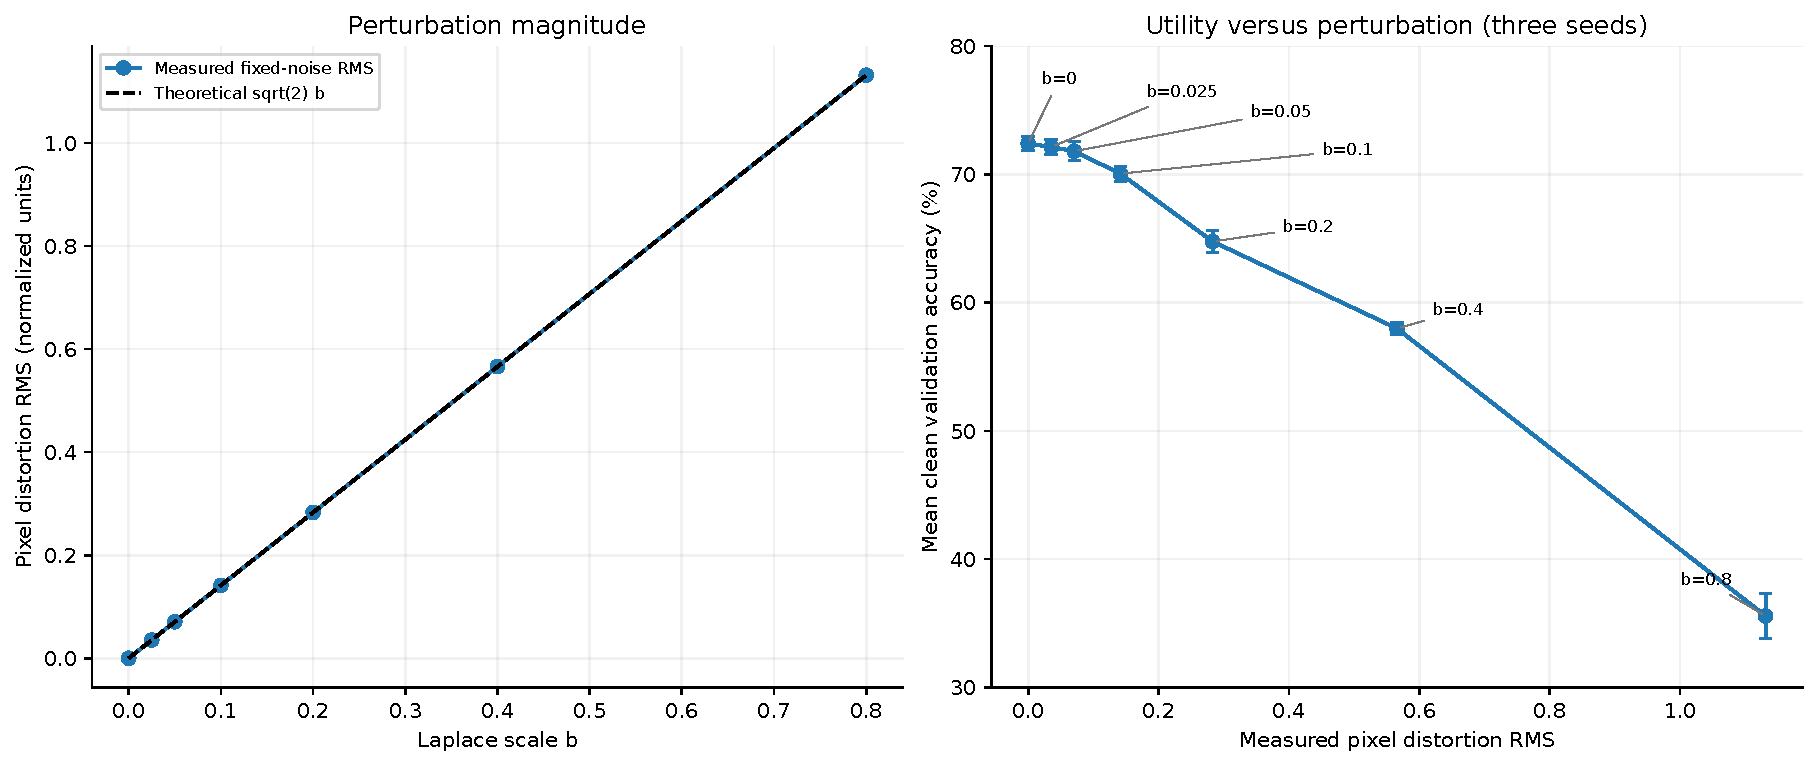
\includegraphics[width=\linewidth]{figures/part2/dp_privacy_utility_tradeoff.pdf}
\caption{Measured RMS distortion versus theory (left), and three-seed mean round-80 clean validation utility versus measured RMS (right). Error bars are sample SD. Annotations identify the tested scales.}\label{fig:distortion}
\end{figure}


\section{Supporting Perturbation Diagnostics}\label{app:noise_diagnostics}
The clean cross-entropy curves complement Question 1's accuracy comparison. The image panel shows how increasing noise alters the same four training images; saturation applies only to display.
\begin{figure}[htbp]
\centering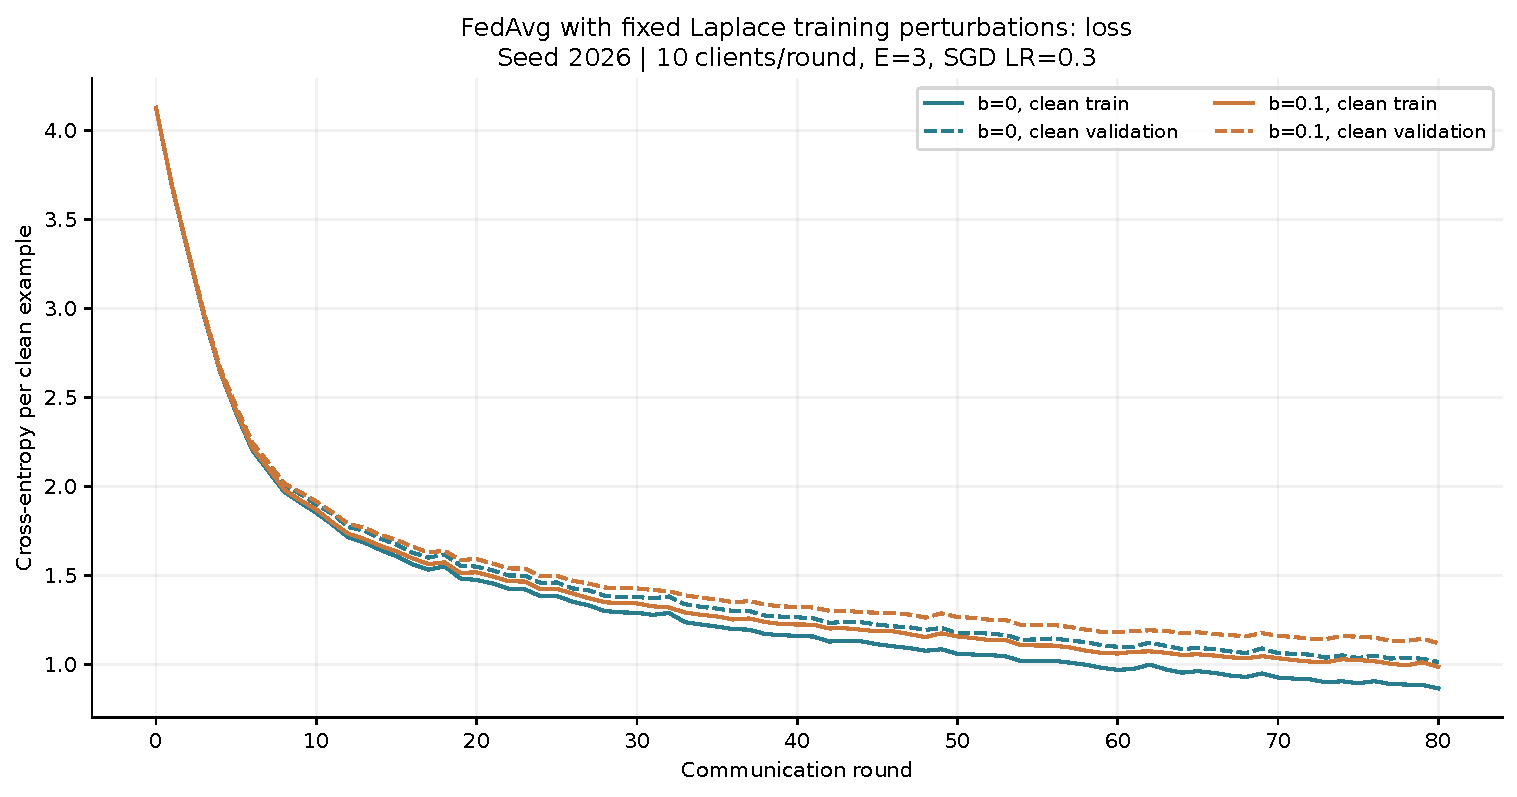
\includegraphics[width=0.9\linewidth]{figures/part2/dp_loss_convergence.pdf}
\caption{Clean-data cross-entropy for the same matched runs as \cref{fig:dpaccuracy}. The positive-noise run learns but retains higher clean training and validation loss. These are evaluation losses, not losses measured on the perturbed local batches.}\label{fig:dploss}
\end{figure}

\begin{figure}[htbp]
\centering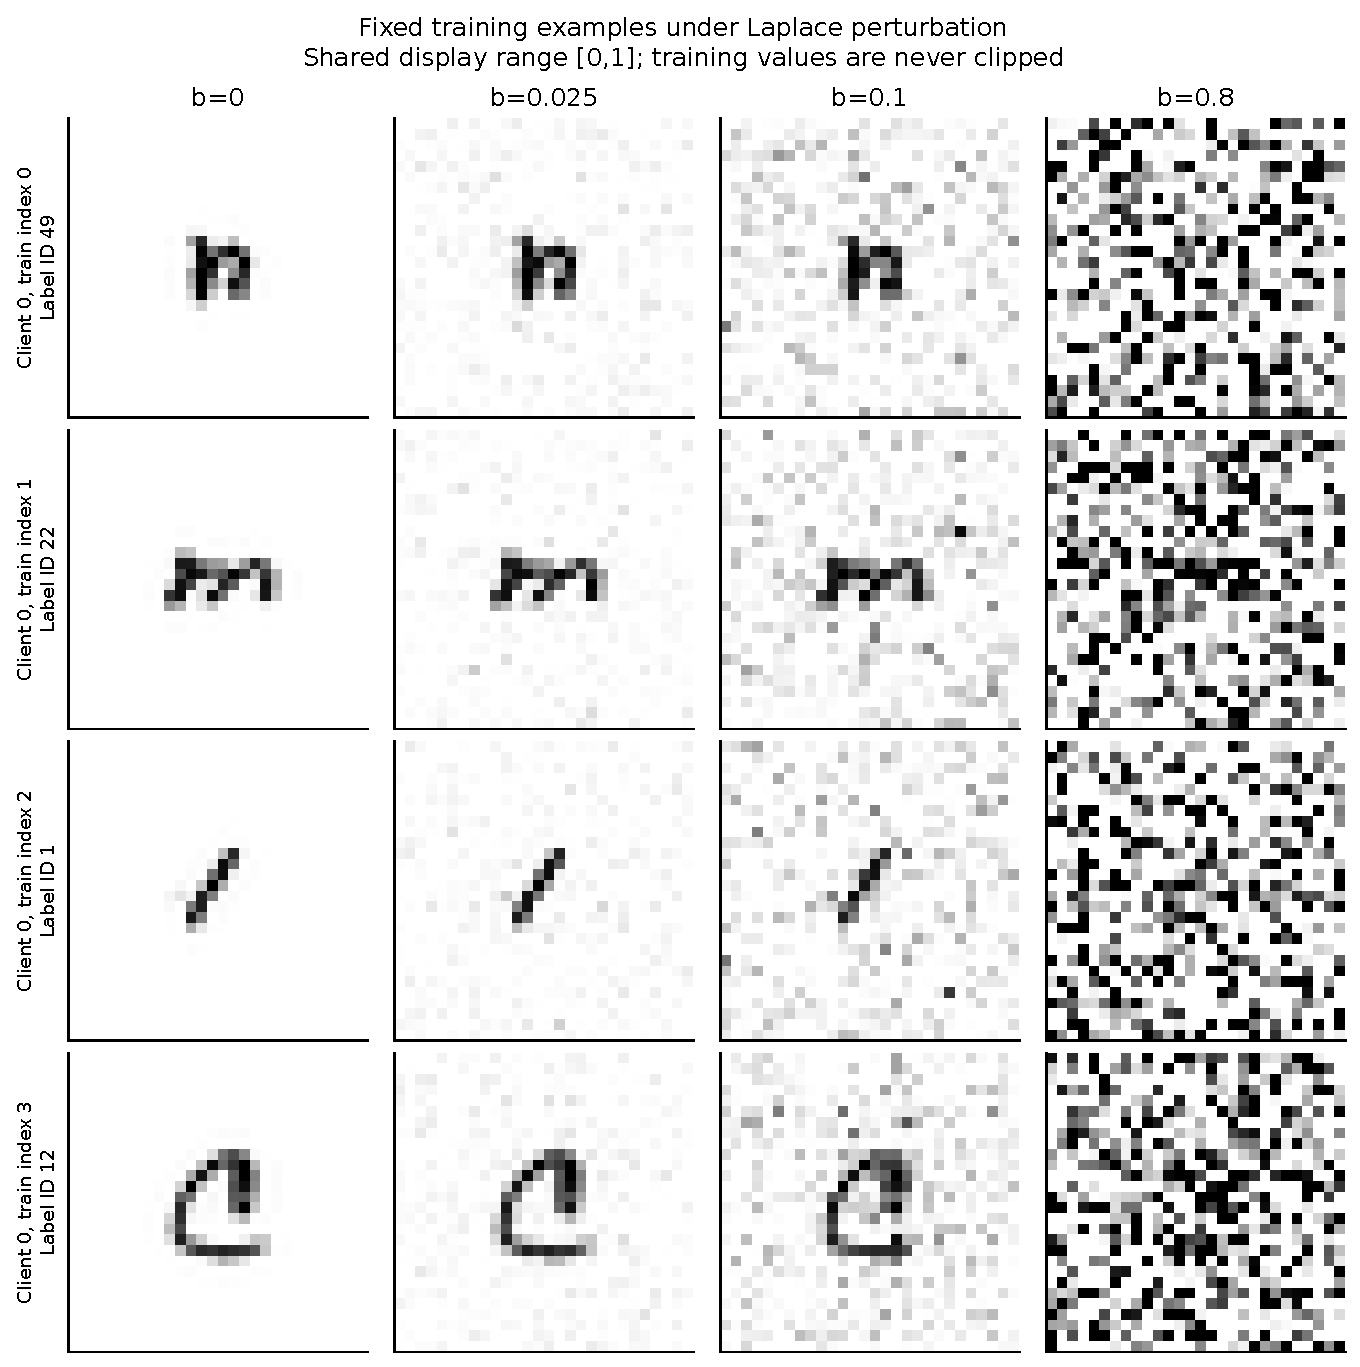
\includegraphics[width=0.76\linewidth]{figures/part2/dp_image_perturbations.pdf}
\caption{Four client-0 training examples at $b=0,0.025,0.10,0.80$, seed 2026. Display values saturate at $[0,1]$; training inputs are never clipped. Labels are numeric class IDs.}\label{fig:images}
\end{figure}

\FloatBarrier
\subsection{Ceiling-limited synthetic noise control}\label{app:synthetic_noise}
A controlled spatial-signal classification task tested whether increasing noise weakens learning. Twenty clients supplied 480 training and 160 validation examples. Seeds 371--373 were each run at $b=0,0.2,2.0$ for 30 rounds, with $E=1$ and learning rate 0.1. All nine runs achieved 100\% clean-validation accuracy across the three noise scales and three seeds. This ceiling effect prevents the task from distinguishing noise-induced degradation and cannot establish robustness to perturbation. The real Federated EMNIST grid in \cref{tab:noisegrid} provides the primary evidence for performance degradation.

\section{All Seed-Specific Final-Round Noise Results}\label{app:allnoise}
\begin{longtable}{rrrrrr}
\caption{All 21 round-80 outcomes. Accuracy is in percent; correct counts refer to the clean held-out test partition.}\label{tab:allnoise}\\
\toprule
$b$ & Seed & Clean train & Clean validation & Test & Correct / 3,621\\
\midrule
\endfirsthead
\toprule
$b$ & Seed & Clean train & Clean validation & Test & Correct / 3,621\\
\midrule
\endhead
\bottomrule\endfoot
0 & 2026 & 75.32 & 73.00 & 74.12 & 2,684\\
0 & 2027 & 74.83 & 72.33 & 72.88 & 2,639\\
0 & 2028 & 74.76 & 71.87 & 73.13 & 2,648\\
0.025 & 2026 & 75.23 & 72.81 & 73.90 & 2,676\\
0.025 & 2027 & 74.64 & 71.89 & 72.80 & 2,636\\
0.025 & 2028 & 74.62 & 71.69 & 72.77 & 2,635\\
0.05 & 2026 & 74.64 & 72.64 & 73.29 & 2,654\\
0.05 & 2027 & 73.80 & 71.39 & 72.27 & 2,617\\
0.05 & 2028 & 74.02 & 71.36 & 72.41 & 2,622\\
0.1 & 2026 & 72.37 & 70.72 & 71.64 & 2,594\\
0.1 & 2027 & 72.01 & 69.74 & 70.67 & 2,559\\
0.1 & 2028 & 72.10 & 69.69 & 70.62 & 2,557\\
0.2 & 2026 & 67.28 & 65.49 & 67.05 & 2,428\\
0.2 & 2027 & 66.54 & 64.94 & 65.84 & 2,384\\
0.2 & 2028 & 65.81 & 63.85 & 65.29 & 2,364\\
0.4 & 2026 & 59.38 & 58.37 & 58.52 & 2,119\\
0.4 & 2027 & 58.41 & 57.42 & 58.44 & 2,116\\
0.4 & 2028 & 58.95 & 58.14 & 59.40 & 2,151\\
0.8 & 2026 & 34.86 & 33.57 & 34.99 & 1,267\\
0.8 & 2027 & 37.65 & 36.88 & 38.66 & 1,400\\
0.8 & 2028 & 37.80 & 36.24 & 37.81 & 1,369\\
\end{longtable}

\Cref{tab:allnoise} gives the seed-specific outcomes underlying \cref{tab:noisegrid}. Each model is evaluated at round 80 on the same 3,621 test examples. Question 1 uses the seed-2026 $b=0.10$ validation-best checkpoint, which also occurs at round 80.

\section{Complete Reproduction Commands}\label{app:reproduction}
These Bash commands run from the repository root after dataset placement and installation of the versions in \cref{sec:methodology}. Select an available GPU through the host's normal allocation procedure. Parts 1.1 and 2 accept \texttt{--device cpu}; reproducing the GPU comparisons requires CUDA. The shared split manifest is reused throughout.

\begin{lstlisting}[language=bash]
export CUBLAS_WORKSPACE_CONFIG=:4096:8 MPLBACKEND=Agg
export OMP_NUM_THREADS=2 MKL_NUM_THREADS=2 OPENBLAS_NUM_THREADS=2
# Part 1.1: data analysis, pilot, grid, and scientific validation
python -m part1_1.run_tests
for phase in inspect pilot suite validate; do
  python -m part1_1 "$phase" --device cuda:0
done
python -m part1_1.audit
# Freeze selection before accessing test data
for phase in select test plots report; do
  python -m part1_1 "$phase" --device cuda:0
done
python -m part1_1.audit --final
\end{lstlisting}
The pilot selects the shared learning rate, the suite includes leading-setting seed repeats, and validation executes the controls in \cref{sec:p11validation}. For a separate configurable run, copy the split manifest into the new output directory first:
\begin{lstlisting}[language=bash]
python -m part1_1 train --device cpu --rounds 80 \
  --fraction 0.10 --epochs 3 --lr 0.3 --batch-size 32 \
  --seed 2026 --threads 2 --name controlled_run \
  --output-dir new_outputs
\end{lstlisting}

Ray requires one thread per process. Preparation creates client-specific training files; validation includes numerical comparisons and three-repeat CPU/GPU benchmarks. Training runs the matched trajectories and evaluates the validation-selected model:
\begin{lstlisting}[language=bash]
export OMP_NUM_THREADS=1 MKL_NUM_THREADS=1 OPENBLAS_NUM_THREADS=1
python -m part1_2.workflow prepare
python -m part1_2.workflow validate
python -m part1_2.extra_validation
python -m part1_2.workflow train
python -m part1_2.workflow artifacts
python -m part1_2.audit
\end{lstlisting}

Part 2 uses the completed Part 1.1 baselines for full zero-noise validation. The scientific phase includes synthetic controls, fixed/resampled-noise ablations, and recovery/stress tests. All 21 final checkpoints and the separate Question 1 checkpoint are evaluated only after the pretest audit and protocol freeze:
\begin{lstlisting}[language=bash]
export OMP_NUM_THREADS=2 MKL_NUM_THREADS=2 OPENBLAS_NUM_THREADS=2
for phase in init math pilot grid science; do
  python -m part2.workflow "$phase" --device cuda:0
done
python -m part2.audit --pretest
python -m part2.workflow freeze
python -m part2.workflow test --device cuda:0
python -m part2.workflow artifacts
python -m part2.workflow audit
\end{lstlisting}
Completed configurations and test results are cached. Fresh repetitions should use separate output/project copies. On interruption, each workflow restores the last committed checkpoint; Part 2 regenerates fixed perturbations from their client keys.
